\begin{appendices}
\cleardoublepage

\chapter{On-line Resources} 
\label{app:code}
An On-line Repository has been created in order to share all of this project's resources, so that researchers and every person interested in the topic can use this information for future work. Code documentation can be found in file: \texttt{Readme.md}. Data documentation can be found in Appendix~\ref{app:dataset}.

\vspace{0.5cm}

\noindent\fbox{%
    \parbox{\textwidth}{%
Link to the On-line repository with code and data:

\url{https://github.com/Marcsiq2/masterthesis}
    }%
}

\vspace{0.5cm}
Also, a few synthesised few synthesised MIDI examples have been uploaded to Soudncloud in order to be accessible to everyone. 

\vspace{0.5cm}

\noindent\fbox{%
    \parbox{\textwidth}{%
Link to Soundcloud:

\url{https://soundcloud.com/marc-siquier-penyafort/sets/master-thesis}
    }%
}

\vspace{0.5cm}
Finally, the On-line survey code can also be found at GitHub:

\vspace{0.5cm}

\noindent\fbox{%
    \parbox{\textwidth}{%
Link to On-line survey repository:

\url{https://github.com/Marcsiq2/Marcsiq2.github.io}
    }%
}
\vspace{0.5cm}


\cleardoublepage

\chapter{Dataset Documentation}
\label{app:dataset}
Data for this thesis can be found at our On-line repository (Appendix~\ref{app:code}) inside the \texttt{Files} folder with the following structure:

\vspace{1cm}
\dirtree{%
.1 Files.
.2 dataOut.
.3 arff.
.3 arff\_cleaned.
.3 nmat.
.2 extracted\_midi.
.3 Darn\_that\_dream.
.3 Suite\_en\_la.
.2 Figures.
.2 guitar\_in.
.3 Darn\_that\_dream.
.3 Suite\_en\_la.
.3 Suite\_en\_la\_v2.
.2 Predictions.
.3 Midis.
.2 scores.
.3 midi.
.3 musescore.
.3 pdf.
.3 xml.
.2 Synth.
.2 weka\_files.
.3 results.
.2 xmlutils.
}

In folder \texttt{dataOut/arff} we can find the arff files for training the models with extracted features and computed performance actions. Arff files inside \texttt{dataOut/arff\_cleaned} are the files used in section~\ref{chap:results} for the evaluation (divided by Onset, Energy and also "All" database files). In folder \texttt{dataOut/nmat} we can find a few Matlab workspaces with all the variables used in the computation.

In folder \texttt{extracted\_midi} we can find transcribed MIDI files from the audio divided by musical piece (both performances of \textit{Suite en la} are inside \texttt{extracted\_midi/Suite\_en\_la} subfolder).

In folder \texttt{Figure} we can find diverse figures used in this written report.

In folder \texttt{guitar\_in} we can find the hexaphonic recordings (a wav file for each string) for each performance.

In folder \texttt{Predictions} we can find csv files with the results of the models. First column indicates note number, second column reference value, third column predicted value and fourth column the error difference. Inside \texttt{Predictions/Midis} subfolder we can find a few re-constructed midis with the predicted values.

In folder \texttt{scores} we can find the scores of the musical pieces in four different formats.

In folder \texttt{Synth} we can find synthesised fragments used for the qualitative evaluation.

In folder \texttt{weka\_files} we can find the experiment description both for the quantitative evaluation and for the feature selection. Inside \texttt{weka\_files/results} we can find output files provided by Weka.

In folder \texttt{xmlutils} we can find a few utils needed in order to be able to read xml files.

\cleardoublepage


\chapter{On-line Survey}
\label{app:survey}
An On-line Survey for the quantitative evaluation was developed using BeaqleJS (browser based evaluation of audio quality and comparative listening environment) which provides a framework to create browser based listening tests and is purely based on open web standards like HTML5 and Javascript.

Server was set in a Github pages account, and can be found at \url{https://marcsiq2.github.io/}.

In Figure~\ref{fig_app:survey_instructions} we can see the starting first page of the survey. This main page shows a few instructions in order to complete the survey as well as my personal contact information. By clicking "Start" the survey starts.

Survey consists of four different listening tests, each one looking like Figure~\ref{fig_app:survey_test}. Three different excerpts are given to the user who can play, pause, rewind and listen to them as many times as he wants. After listening to all of them he is asked to rate \textit{How much "human" are the audios?} from Bad to Excellent by using a slider for each one, so no numerical value is given by the user. By navigating with "Previous Test" and "Next test" he can go back and forth in order to change ratings if he needs to.

After completing the four different tests (12 excerpts in total) the user is presented with the "Submit" page (Figure~\ref{fig_app:survey_end}), were he can input his own name and email or write any comment about the test. Those fields are not mandatory. Not many comments were given and the most meaningful one is \textit{I based my "humanness" mainly in the attack of the instrument, when the time between one attack and the next is really short, it feels robotic and hasty. I tried not to guide myself on synthesis but it is difficult. The best of my grades went to a somehow "slower" performance with more rallentando than the other versions.}.

In Table~\ref{tab:survey_results} we can see the punctuation given to each excerpt by each one of the 12 users. This punctuation is directly mapped from the rating slider, being hard right 100 points and hard left 0 points. 

In Figure~\ref{fig_app:survey} we can see those punctuations merged by type (Performance, Prediction and Score synthesis) and in Figure~\ref{fig_app:survey_test2} punctuations are divided and plotted by test number.

In Figure~\ref{fig_app:survey_runtime} and as a curiosity we can see a runtime plot for each one of the four different tests, being \textit{intro\_1} the test with higher average runtime.

\begin{figure}[ht!]
\centering 
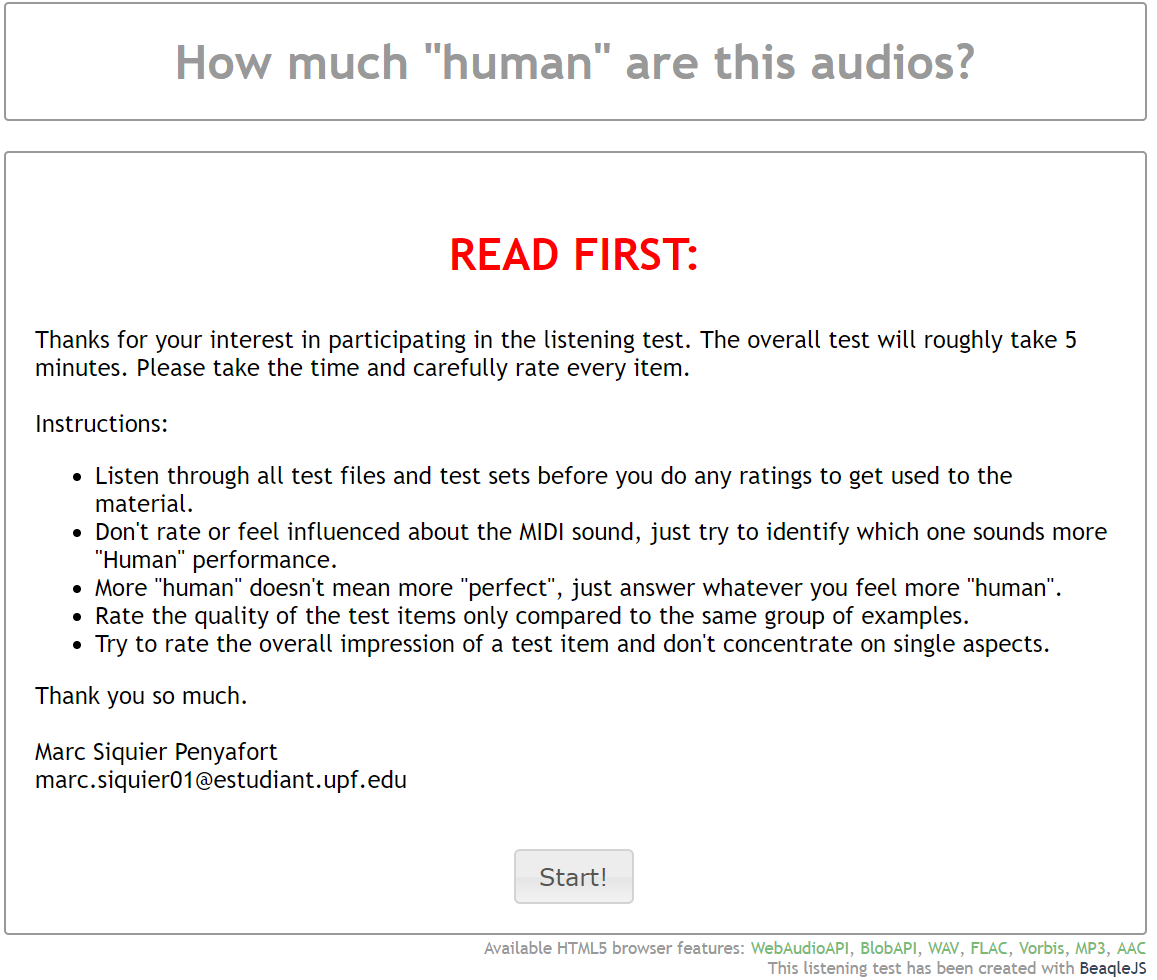
\includegraphics[width=0.8\textwidth]{Figures/survey_instructions.PNG}
\caption{On-line survey instructions.}
\label{fig_app:survey_instructions}
\end{figure}

\begin{figure}[ht!]
\centering
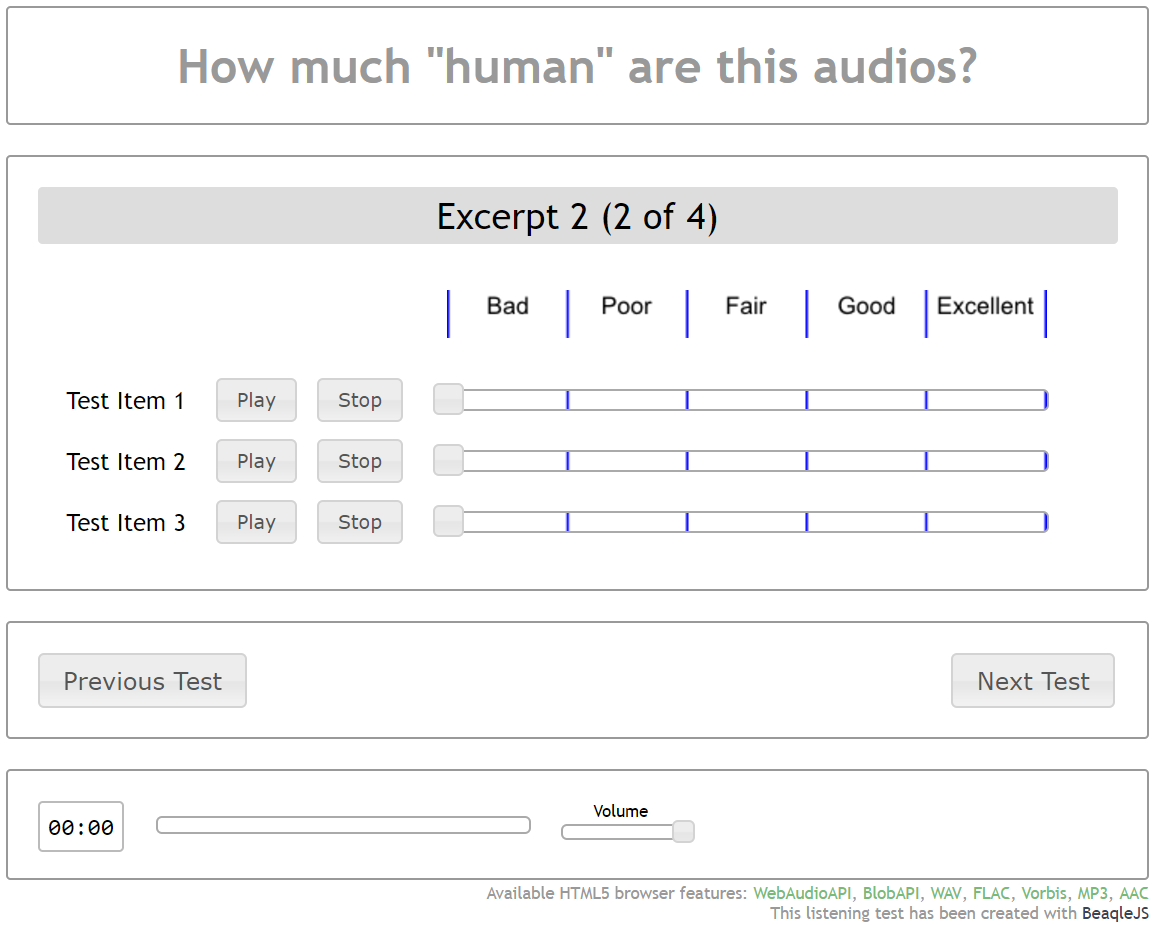
\includegraphics[width=0.8\textwidth]{Figures/survey_test.PNG}
\caption{On-line survey example of a Test set.}
\label{fig_app:survey_test}
\end{figure}

\begin{figure}[ht!]
\centering
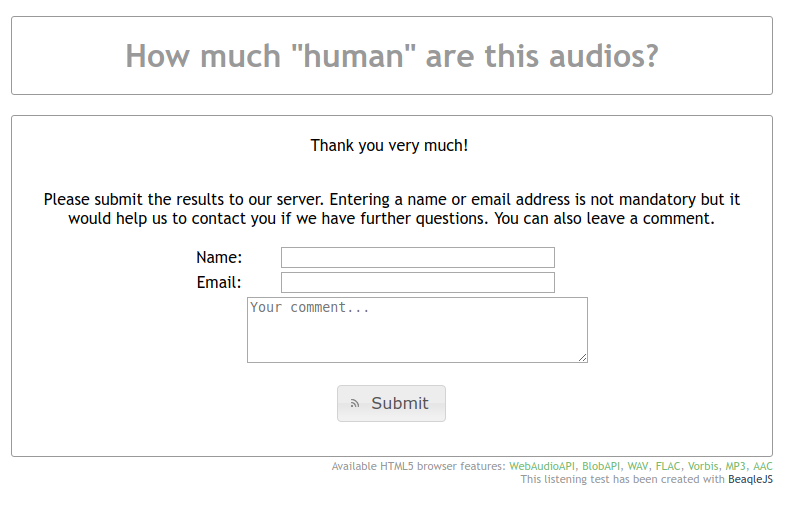
\includegraphics[width=0.8\textwidth]{Figures/survey_end.png}
\caption{On-line survey submit page.}
\label{fig_app:survey_end}
\end{figure}

\begin{table}[ht!]
\centering
  \caption[Full table results of the on-line survey.]{Full table results of the on-line survey.}
  \label{tab:survey_results}
  \footnotesize
\begin{tabular}{l|ccc|ccc|ccc|ccc}

\hline
\multicolumn{1}{c}{\multirow{2}{*}{}} & \multicolumn{3}{c}{intro1} & \multicolumn{3}{c}{intro2} & \multicolumn{3}{c}{middle}  & \multicolumn{3}{c}{end} \\ 
\multicolumn{1}{c}{}                      & \multicolumn{1}{c}{Perf} & \multicolumn{1}{c}{Pred} & \multicolumn{1}{c}{Score} & \multicolumn{1}{c}{Perf} & \multicolumn{1}{c}{Pred} & \multicolumn{1}{c}{Score} & \multicolumn{1}{c}{Perf} & \multicolumn{1}{c}{Pred} & \multicolumn{1}{c}{Score} & \multicolumn{1}{c}{Perf} & \multicolumn{1}{c}{Pred} & \multicolumn{1}{c}{Score} \\ \hline
1 & 20 & 51 & 43 & 63 & 43 & 83 & 40 & 26 & 75 & 75 & 34 & 40 \\ 
2 & 31 & 29 & 76 & 73 & 33 & 91 & 13 & 29 & 52 & 13 & 25 & 88 \\ 
3 & 61 & 39 & 62 & 48 & 35 & 69 & 57 & 30 & 61 & 45 & 47 & 62 \\
4 & 49 & 49 & 55 & 63 & 43 & 83 & 29 & 66 & 76 & 45 & 67 & 78 \\
5 & 46 & 37 & 50 & 45 & 47 & 81 & 70 & 50 & 76 & 40 & 37 & 80 \\ 
6 & 35 & 69 & 26 & 70 & 65 & 50 & 39 & 70 & 50 & 32 & 91 & 68 \\
7 & 50 & 71 & 49 & 50 & 50 & 50 & 68 & 54 & 87 & 35 & 68 & 69 \\
8 & 33 & 72 & 50 & 70 & 71 & 29 & 66 & 68 & 47 & 90 & 47 & 68 \\
9 & 40 & 19 & 53 & 49 & 61 & 72 & 49 & 30 & 49 & 20 & 9 & 52 \\
10 & 31 & 12 & 50 & 66 & 46 & 96 & 51 & 63 & 67 & 44 & 66 & 88 \\ 
11 & 57 & 30 & 65 & 42 & 31 & 62 & 38 & 32 & 69 & 45 & 34 & 61 \\ \hline                  
\end{tabular}

\end{table}

\begin{figure}
\centering
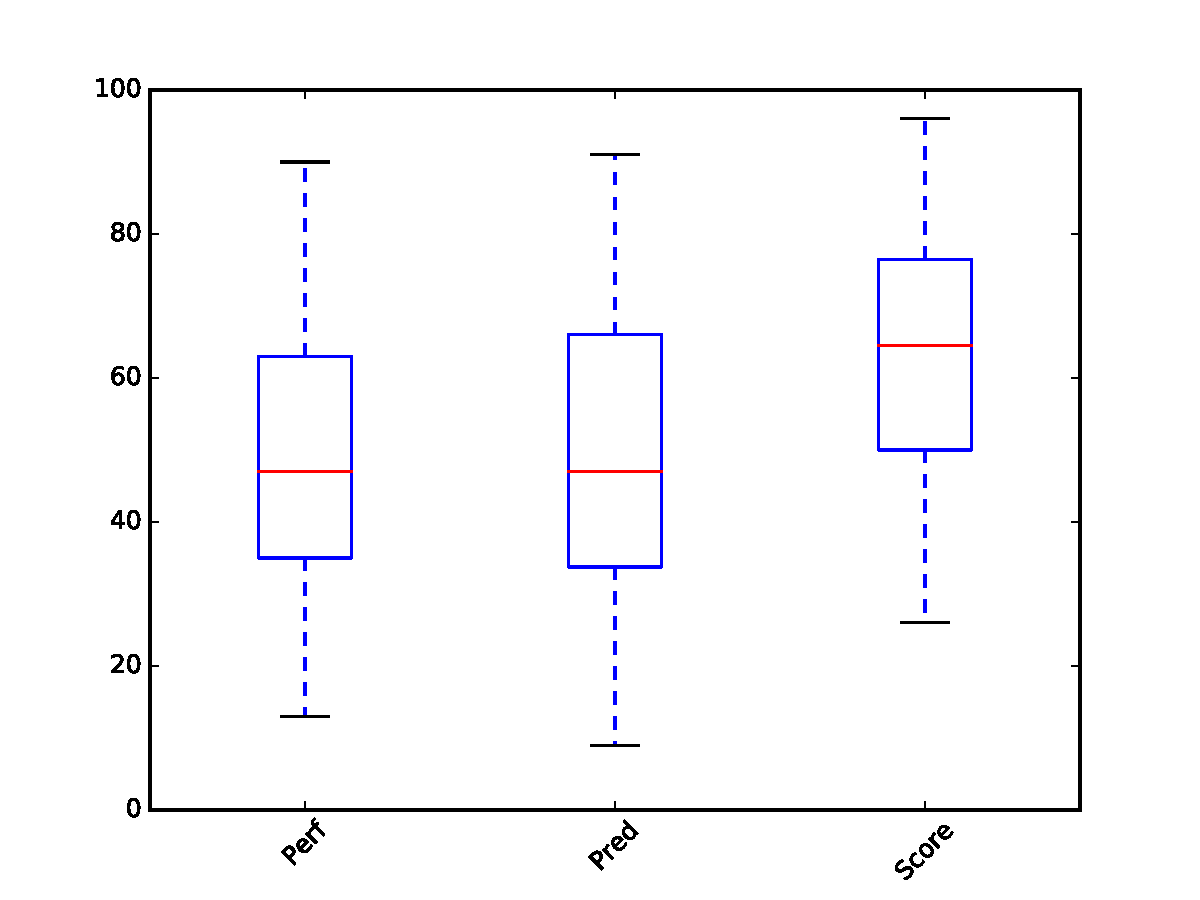
\includegraphics[width=0.8\textwidth]{Figures/survey.pdf}
\caption{Results of the on-line survey with performance, predicted and straight score synthesised midis.}
\label{fig_app:survey}
\end{figure}

\begin{figure}
\centering
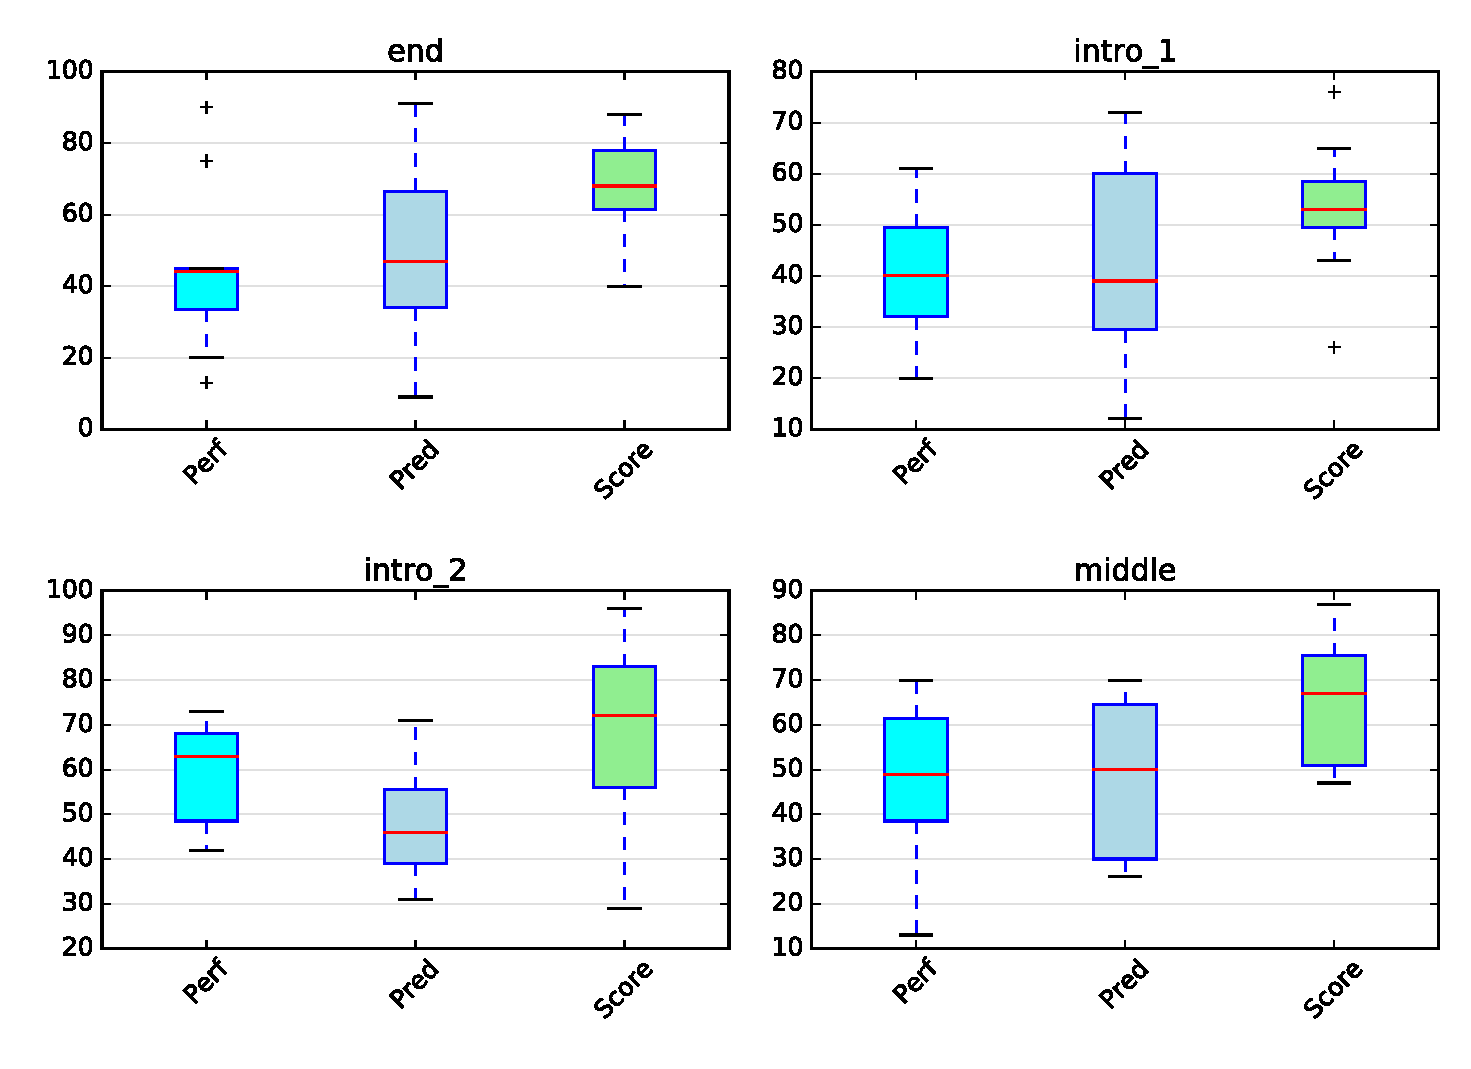
\includegraphics[width=0.8\textwidth]{Figures/survey_tests.pdf}
\caption{Results per test of the on-line survey with performance, predicted and straight score synthesised midis.}
\label{fig_app:survey_test2}
\end{figure}

\begin{figure}
\centering
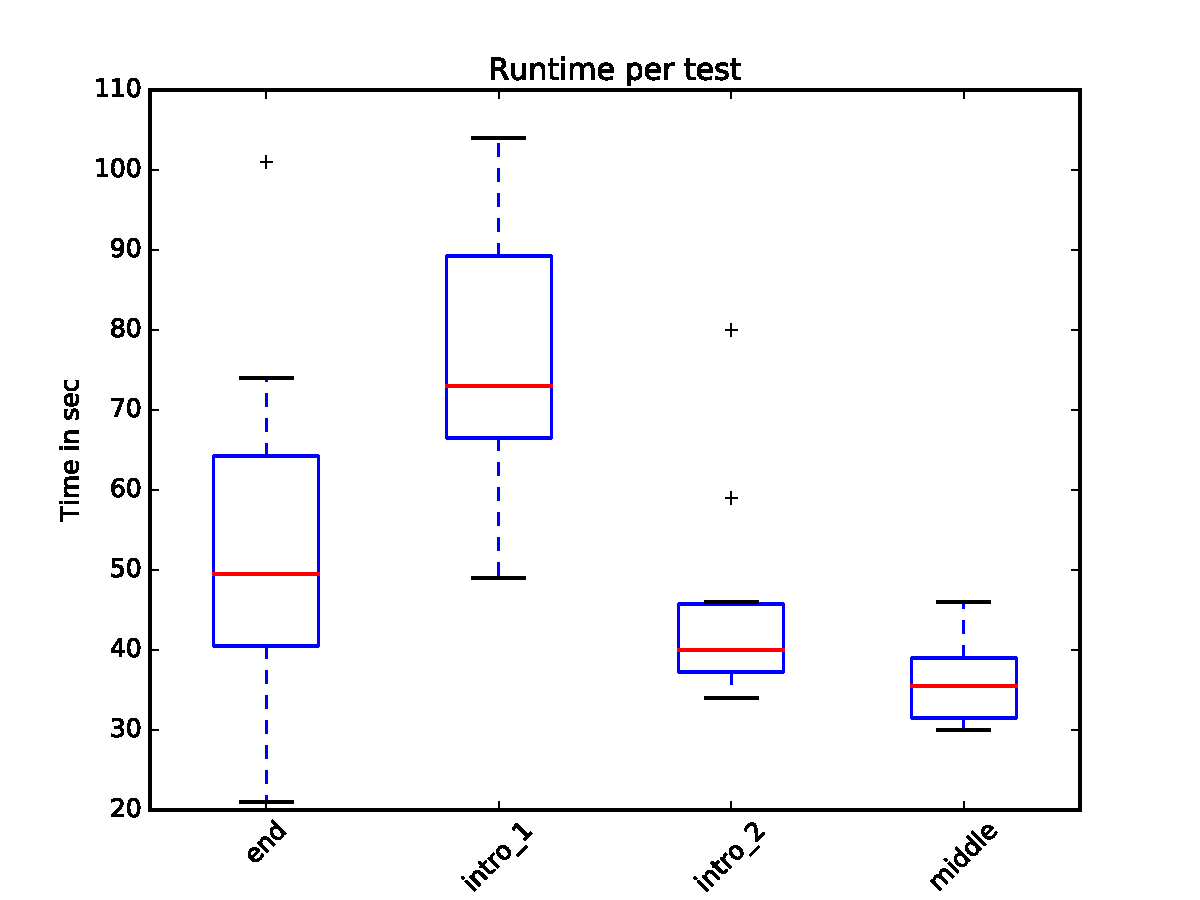
\includegraphics[width=0.8\textwidth]{Figures/survey_runtime.pdf}
\caption{Runtime for each test of the on-line survey.}
\label{fig_app:survey_runtime}
\end{figure}

\cleardoublepage

\end{appendices}

